\documentclass[12pt]{article}
% =====================================================================
%  wpstyle.tex — 共用工作論文版式（XeLaTeX）
%  單欄 A4｜booktabs 三線表｜無彩色｜Noto Serif TC
%  編譯：xelatex f ; xelatex f ; python3 fixtounicode.py f.pdf
% =====================================================================
\usepackage{geometry}
\geometry{a4paper,left=2.9cm,right=2.9cm,top=3.0cm,bottom=3.0cm}

\usepackage{fontspec}
\setmainfont{Noto Serif TC}[
  BoldFont       = Noto Serif TC,
  ItalicFont     = Noto Serif TC,
  BoldItalicFont = Noto Serif TC,
  Ligatures      = TeX]
\setsansfont{Noto Sans TC}[BoldFont=Noto Sans TC]
\setmonofont{Consolas}[Scale=0.90]

\XeTeXlinebreaklocale "zh"
\XeTeXlinebreakskip = 0pt plus 0.06em minus 0.02em

\usepackage{amsmath,amssymb}
\usepackage{booktabs}
\usepackage{array}
\usepackage{longtable}
\usepackage{tabularx}
\usepackage{multirow}
\usepackage{graphicx}
\usepackage{setspace}
\usepackage{ragged2e}
\usepackage{enumitem}
\setlist{leftmargin=2.2em,topsep=4pt,itemsep=2pt,parsep=0pt}

\usepackage[hang,flushmargin,bottom]{footmisc}
\setlength{\footnotemargin}{1em}

\usepackage[labelsep=period,font=small,labelfont=bf,justification=justified]{caption}
\captionsetup[table]{skip=4pt,position=top}
\captionsetup[figure]{skip=6pt,position=bottom}

\usepackage{titlesec}
\titleformat{\section}{\normalfont\bfseries\large}{\thesection}{0.7em}{}
\titleformat{\subsection}{\normalfont\bfseries\normalsize}{\thesubsection}{0.7em}{}
\titleformat{\subsubsection}{\normalfont\bfseries\small}{\thesubsubsection}{0.7em}{}
\titlespacing*{\section}{0pt}{2.4ex plus .6ex}{1.2ex}
\titlespacing*{\subsection}{0pt}{1.9ex plus .5ex}{0.85ex}
\titlespacing*{\subsubsection}{0pt}{1.5ex plus .4ex}{0.7ex}

\usepackage[hidelinks,unicode,breaklinks=true]{hyperref}
\hypersetup{colorlinks=false,pdfborder={0 0 0}}
\usepackage{url}
\urlstyle{tt}
\Urlmuskip=0mu
\def\UrlBreaks{\do\/\do.\do=\do?\do\&\do\_}

\usepackage{natbib}
\bibpunct{(}{)}{;}{a}{}{,}
\setlength{\bibsep}{2.5pt plus 0.3ex}

\setlength{\parindent}{2em}
\setlength{\parskip}{0pt}
\renewcommand{\baselinestretch}{1.22}
\renewcommand{\arraystretch}{1.18}
\setlength{\tabcolsep}{5pt}
\setlength{\skip\footins}{5mm}
\setlength{\emergencystretch}{1.5em}
\hyphenpenalty=1500
\tolerance=1500

\usepackage{fancyhdr}
\pagestyle{fancy}\fancyhf{}
\renewcommand{\headrulewidth}{0pt}
\fancyfoot[C]{\small\thepage}
\fancypagestyle{plain}{\fancyhf{}\renewcommand{\headrulewidth}{0pt}\fancyfoot[C]{\small\thepage}}

\newcommand{\wptitle}[1]{{\centering\bfseries\LARGE #1\par}\vspace{0.6em}}
\newcommand{\wpsubtitle}[1]{{\centering\large #1\par}\vspace{1.8em}}
\newcommand{\wpauthor}[2]{{\centering\large #1\par\vspace{0.4em}{\small #2}\par}\vspace{1.1em}}
\newcommand{\wpdate}[1]{{\centering\small #1\par}\vspace{2.0em}}

\newenvironment{wpabstract}
  {{\centering\bfseries 摘\quad 要\par}\vspace{0.4em}%
   \begin{quote}\small\setlength{\parindent}{1.8em}}
  {\end{quote}\vspace{0.5em}}

\newcommand{\keywords}[1]{\begin{quote}\small\noindent\textbf{關鍵詞}：#1\end{quote}\vspace{-0.4em}}
\newcommand{\jel}[1]{\begin{quote}\small\noindent\textbf{JEL 分類}：#1\end{quote}}

\newenvironment{tabnote}[1][\linewidth]
  {\par\vspace{3pt}\begin{minipage}{#1}\footnotesize\setlength{\parindent}{0pt}\textbf{說明}：}
  {\end{minipage}\par\vspace{2pt}}

\newcommand{\ttt}[1]{\texttt{\small #1}}


\newcommand{\MainGrowth}{4.61}
\newcommand{\HourlyGrowth}{15.56}
\newcommand{\HoursGap}{10.95}
\newcommand{\MainWithin}{2525}
\newcommand{\MainShift}{-12}
\newcommand{\MainInteraction}{-407}
\newcommand{\MainTotal}{2107}
\newcommand{\CounterfactualGap}{418}
\newcommand{\ShiftPValue}{0.958}
\newcommand{\ChainWithin}{2364}
\newcommand{\ChainShift}{-229}
\newcommand{\ChainInteraction}{-28}
\newcommand{\InteractionShrink}{93.02}
\newcommand{\ChainMethodGap}{28}
\newcommand{\IndustryTopThree}{73.46}
\newcommand{\TotalGrowth}{11.11}
\newcommand{\OfficialRegularGrowth}{3.96}
\newcommand{\OfficialTotalGrowth}{10.26}
\newcommand{\RegularOfficialGap}{-0.66}
\newcommand{\TotalOfficialGap}{-0.84}

\begin{document}

\wptitle{台灣實質薪資停滯的分解}
\wpsubtitle{產業內成長、結構移轉、工時與薪資組成}
\wpauthor{楊世永}{獨立研究者；\href{mailto:sheyung21@gmail.com}{sheyung21@gmail.com}}
\wpdate{2026 年 8 月 9 日}

\begin{wpabstract}
本文以行政院主計總處二○○○至二○二四年工業及服務業資料，將共同十六行業的實質平均薪資變動分為產業內、就業占比移轉與交乘項。實質經常性月薪對數成長僅 \MainGrowth\%，時薪成長則為 \HourlyGrowth\%，差距達 \HoursGap 個百分點。端點 Laspeyres 分解的月薪增加額為新臺幣 \MainTotal 元，其中產業內為 \MainWithin 元、移轉為 \MainShift 元、交乘為 \MainInteraction 元；端點交乘在 Paasche 下改為正值，顯示基期選擇敏感。逐年連鎖後，產業內、移轉與交乘累積額分別為 \ChainWithin、\ChainShift 與 \ChainInteraction 元，交乘絕對值及兩方法的產業內差距均縮減 \InteractionShrink\%。三年循環區塊自助法的一萬次抽樣顯示，二○二四年累積總變動的百分之九十五區間為負三八三○至八五一五元，區間寬度大於觀察變動；端點產業內區間亦跨零，移轉雙尾值為零點九五八，故不得賦予傳統推論意義。研究者看過全期端點後提出的三項條件式事前預測均獲資料支持：二○一九至二○二一年移轉為正、二○二二至二○二四年反轉為負，月薪與時薪成長差在疫情前兩年擴大。六個制度分段的年均變動正負交替，端點與連鎖合計相同而配置略異，因此事件年份只作描述邊界，不視為政策斷點。固定二○○○年占比的二○二四年反事實薪資高四一八元，與負向淨移轉一致。產業內成長高度集中，前三大行業占絕對貢獻 \IndustryTopThree\%；總薪資成長 \TotalGrowth\%，快於經常性薪資。官方發布實質序列的經常性與總薪資成長為 \OfficialRegularGrowth\% 與 \OfficialTotalGrowth\%，和共同樣本相差 \RegularOfficialGap 與 \TotalOfficialGap 個百分點，幾乎全由共同樣本界定解釋。部分工時人數無全期一致序列，故不設代理變數。全部結果是可重現的描述性會計，不識別制度或產業結構的因果效果。
\end{wpabstract}

\keywords{實質薪資；shift-share；產業結構；工作時數；台灣}
\jel{J31；J21；C43}

\section{緒論}

台灣薪資停滯的公共討論常把兩個機制混在一起：一是各產業內部的薪資成長偏慢，二是受僱員工逐漸移往不同薪資水準的產業。兩者的政策含義不同。若前者為主，問題較接近廣泛的生產力、議價、報酬分配與價格調整；若後者重要，產業組成、職務配置與部門移動便更關鍵。然而總體平均薪資同時受產業薪資與就業權數變動影響，僅比較總體序列無法區分兩者。

本文建立一套可完全重現的描述性分解。第一，使用官方受僱員工人數作權數，對實質經常性薪資與總薪資同時執行 Laspeyres、Paasche 與 Törnqvist 分解，完整保留交乘或近似殘差。第二，將月薪除以一致的正常或總工時，量化月薪與時薪成長差。第三，在同一發布版次內比較大類與中類，避免把官方後續修訂誤認為分類粒度效果。第四，建立固定期初受僱人數占比的反事實路徑。第五，用跨年的共同區塊 bootstrap 描述分量對時間抽樣的敏感度。

主要發現有三點。其一，2000--2024 年共同樣本的實質經常性月薪只增加 \MainGrowth\%，但時薪增加 \HourlyGrowth\%；工作時數變動是兩種衡量差距的重要會計來源。其二，不論基期公式，產業內薪資變動遠大於純結構移轉；結構分量的符號與交乘分配會隨基期而改變，故不應只報單一版本。其三，中類化確實改變各分量，但不支持「分類愈細，產業內分量必然愈小」的單調敘事。

本文的貢獻不在因果識別，而在證據邊界：同時固定資料版本、涵蓋範圍、價格基期、分類接縫與會計公式，讓「結構」一詞只承擔資料可支持的含義。所有下載網址、SHA-256、排除紀錄、結果表與論文數字均由公開 repository 中的固定腳本產生。

\section{資料與涵蓋範圍}

\subsection{官方來源}

核心資料來自主計總處《薪資與生產力統計年報》\citep{dgbas-yearbook}。年報說明其資料係按月蒐集各業場所受僱員工人數、薪資與工時後彙編；本文使用歷年各業受僱員工人數、每人每月總薪資、每人每月經常性薪資及每人每月工作時數四組表。2019 年發布版補足 2000--2004 年，2024 年發布版提供 2005--2024 年最新版回溯序列。2016--2024 年中類資料則逐年使用當期年報，共 378 個官方工作簿。資料開放平臺亦將薪資年報列為免費、免申請的原始資料集\citep{dgbas-wage}。

消費者物價使用主計總處「消費者物價基本分類指數」月資料的總指數原始值，先取十二個月算術平均，再重標為 2024 年等於 100。所有薪資均以 2024 年新臺幣表示。分類文件包括第 7 至第 11 次行業標準分類的官方新舊對照表；主樣本大類使用共同章別，第 10 與第 11 次分類之間的中類結果分段呈現，不以結果反推一對多的拆分權重\citep{dgbas-class}。

\begin{table}[htbp]
\caption{核心資料與分析用途}
\centering\small
\begin{tabularx}{\textwidth}{p{3.2cm}p{2.5cm}Xp{2.3cm}}
\toprule
資料 & 期間 & 用途 & 分類處理 \\
\midrule
歷年各業受僱員工人數 & 2000--2024 & 大類權數與官方總體重算 & 第 10／11 次共同章別 \\
歷年各業經常性、總薪資 & 2000--2024 & 月薪分解與薪資組成比較 & 同上 \\
歷年各業正常、總工時 & 2000--2024 & 經常性、總時薪 & 同上 \\
逐年中類年報表 & 2016--2024 & 粒度比較 & 修訂內分段 \\
消費者物價總指數 & 2000--2024 & 轉為 2024 年價格 & 2024=100 \\
\bottomrule
\end{tabularx}
\begin{tabnote}
原始來源共 424 筆，每筆的網址、取得日、位元組數、SHA-256、涵蓋期與分類版本記錄於 \ttt{data/source\_manifest.csv}。
\end{tabnote}
\end{table}

\subsection{年度化與結果變數}

官方歷年表已提供完整曆年的十二月平均，避免總薪資受年終獎金發放月份左右。經常性時薪定義為經常性月薪除以正常工時；總時薪定義為總月薪除以總工時。本文不把單月總薪資用於主要分解。

2000--2008 年教育業為「－」，表註並說明 2009 年起才納入教育輔助及其他教育業；2019 年又增加研究發展服務業、學前教育與社會工作服務業。這些是涵蓋變更，不是零就業。主 2000--2024 與 2008--2024 端點分解因此固定在兩端均存在的 16 個大類；2016--2024 使用 17 類。完整官方總體仍逐年重算並作外部一致性檢查，涵蓋擴增不被歸為經濟性的結構移轉。

\subsection{一致性閘門}

對每年與每個必要定義，本文以分業人數重算
\[
\widehat W_t=\frac{\sum_i L_{it}w_{it}}{\sum_i L_{it}},
\qquad
e_t=\frac{|\widehat W_t-W_t^{\mathrm{official}}|}{|W_t^{\mathrm{official}}|}.
\]
最新版大類對官方總體、同版次大類對官方總體，以及中類對同版次大類，共 15 組檢查均通過 0.5\% 門檻。所有組合中的最大相對誤差為 0.052\%，來自工時的小數位四捨五入。薪資最大誤差低於 0.003\%。因此資料在進入分解前通過預先指定的外部閘門。

\subsection{官方實質序列與部分工時可用性}

除行業表自行加權的共同樣本外，本文另從主計總處「薪情平臺」擷取同一薪資調查發布的每人每月實質經常性與實質總薪資年序列\citep{dgbas-platform}。平台顯示的 2000--2024 年序列採官方發布時的消費者物價指數基準；為比較水準，圖中依 2024 年名目薪資等比例換算成 2024 年幣值，但成長率不受這項等比例換算影響。這個外部序列與共同 16 行業加權值不是同一估計量：前者涵蓋官方當年發布範圍，後者刻意固定在全期皆可觀測的行業集合。

薪情平臺也列有「部分工時員工」篩選項。本文實際查詢 2000--2024 年年度受僱人數，結果沒有全期一致的可用值。因此，部分工時比率不進入實證表，也不以住宿餐飲業占比或低工時行業占比代替。這個決定避免把產業結構代理誤寫成僱用型態機制；可用性查核與未納入理由完整保留於結果表 17。

\section{方法}

\subsection{端點分解}

令 $s_{it}=L_{it}/\sum_jL_{jt}$，$w_{it}$ 為某一實質薪資定義，總體平均為 $W_t=\sum_i s_{it}w_{it}$。Laspeyres 型分解為
\[
\Delta W=\sum_i s_{i0}\Delta w_i+\sum_i w_{i0}\Delta s_i+\sum_i\Delta s_i\Delta w_i.
\]
三項依序稱為產業內、結構移轉與交乘。Paasche 型改以期末權數評價：
\[
\Delta W=\sum_i s_{i1}\Delta w_i+\sum_i w_{i1}\Delta s_i-\sum_i\Delta s_i\Delta w_i.
\]
交乘符號反轉，凸顯其分配取決於基期。這類分解是 Kitagawa 型會計恆等式\citep{kitagawa1955}，常見於跨單位加權平均變動的分析；其結構與生產力文獻的 Baily--Hulten--Campbell 分解所區分的 within、between、entry 與 exit 類似\citep{baily1992}，但本文的單位是行業大類而非工廠，且共同樣本不把分類涵蓋變更當成進出。這些恆等式不提供反事實因果效果。

Törnqvist 規格以薪資總額占比 $\theta_{it}=s_{it}w_{it}/W_t$ 及端點平均權重 $\bar\theta_i$ 分解：
\[
\Delta\log W\approx
\sum_i\bar\theta_i\Delta\log w_i+
\sum_i\bar\theta_i\Delta\log s_i.
\]
近似殘差單獨列示。所有可加總版本均以機器測試檢查恆等式，容許誤差為 $10^{-10}$。

\subsection{年度連鎖分解}

端點公式把 24 年的占比與薪資變動一次相乘，交乘項容易吸收基期距離。修訂規格因此把每一相鄰年度視為一個連結。年度 Laspeyres 連結為
\[
W_t-W_{t-1}=\sum_i s_{i,t-1}\Delta w_{it}
+\sum_i w_{i,t-1}\Delta s_{it}
+\sum_i\Delta s_{it}\Delta w_{it},
\]
而累積產業內、移轉與交乘項分別把 2001 年至 $t$ 年的年度連結相加。Paasche 連結改用當期權數與當期薪資，交乘項符號反向。每一年與每個累積端點都直接檢查三分量之和等於 $W_t-W_0$，絕對與相對容許誤差均為 $10^{-10}$。如果年度變動幅度較小，交乘項以及 Laspeyres--Paasche 配置差異應比端點分解縮小；這是一項方法診斷，不是經濟機制的先驗限制。

連鎖路徑的區間仍採三年循環移動區塊 bootstrap：從 24 組年度對數差分抽取連續區塊，循環到序列開頭，重建每個行業的受僱人數與實質薪資路徑，再對每個累積年度重新分解。重複 10,000 次，亂數種子固定為 20260809。圖中的陰影是各累積分量逐年的百分位數區間；若區間寬度大於觀察到的累積變動，圖說直接標示該路徑與零不可區分。

\subsection{制度分段與條件式事前預測}

制度分段以 2002、2009、2017、2020 與 2022 為界。2002 對應台灣自 1 月 1 日成為 WTO 會員\citep{wto2002}；2009 對應全球金融危機後的衰退與緩慢復甦\citep{imf2009}；2017 與 2018 分別標示週休二日修法主要條文生效與後續修法自 3 月 1 日施行\citep{mol2016,mol2018}；2020 對應台灣於 1 月確認首例 COVID-19 境外移入病例\citep{taiwancdc2020}。六段為 2000--2002、2002--2009、2009--2017、2017--2020、2020--2022 與 2022--2024；各段等權呈現端點、連鎖及年平均變動，不把事件邊界視為因果斷點。

在任何第二階段計算前，本文已把三項方向性預測寫入 \ttt{PREANALYSIS.md} 並獨立提交：2019--2021 年結構移轉為正，2022--2024 年反轉為負，以及月薪與時薪成長差在 2020--2021 年擴大。由於研究者已看過 2000--2024 全期端點結果，本文一律稱其為「條件式事前預測（研究者已觀察全期端點結果）」，不用「事前註冊預測」或樣本外檢驗等措辭。

\subsection{分類粒度、工時與反事實}

粒度比較只在同一分類制度、同一發布版次與相同中類共同樣本內進行。中類先直接分解，再將同一批中類按官方年報表組加總為 14 個共同大組後重算大類版本；兩者總變動因而完全相同，差異只反映分組粒度。

固定結構反事實為
\[
W_t^{cf}=\sum_i s_{i0}w_{it}.
\]
本文分別固定 2000、2008 與 2016 年占比。月薪與時薪的會計差以累積對數成長差表示。先分解再平減的敏感度則把名目分解分量以期末價格尺度轉換，並把共同 CPI 變動另列為價格橋接項。

\subsection{不確定性}

本文區分三種不確定性。第一是\textbf{時間路徑變異}：以長度三年的循環移動區塊 bootstrap 衡量年度差分重新排列後的分解敏感度。為保留正值，重抽的是就業與薪資的年度對數一階差分；所有產業共同抽取同一批年份區塊，以保留同期共變動。重複 10,000 次，亂數種子固定為 20260809。第二是\textbf{官方抽樣誤差}：原始發布表沒有逐業共變異矩陣，本文不能重建官方抽樣設計的標準誤。第三是\textbf{規格與涵蓋不確定性}：包括分類版本、共同樣本、端點、薪資口徑、CPI 基準與分解權數，本文用明列的敏感度規格而非單一區間處理。

因此，bootstrap 陰影只回答「若觀察到的年度路徑是可重抽的時間序列，累積會計分量多敏感」，不回答母體參數、抽樣設計或制度效果的不確定性。本文仍報告雙尾比例作描述，但不把它稱為傳統假設檢定；區間跨零只表示此重抽設計下與零不可區分。

\section{結果}

\subsection{月薪與時薪走勢}

圖~\ref{fig:monthly-hourly} 顯示，2000 年共同樣本的實質經常性月薪為 44,647 元，2024 年為 46,754 元，累積對數成長僅 \MainGrowth\%。相同薪資分子除以正常工時後，實質經常性時薪由 248.6 元上升至 290.5 元，累積成長 \HourlyGrowth\%；金額為四捨五入顯示，成長率由未捨入值計算。兩者差 \HoursGap 個對數百分點，與正常工時下降的會計效果一致。這不表示縮短工時「造成」生產力或福利變化，只表示月薪停滯比時薪停滯更明顯。

\begin{figure}[htbp]
\centering
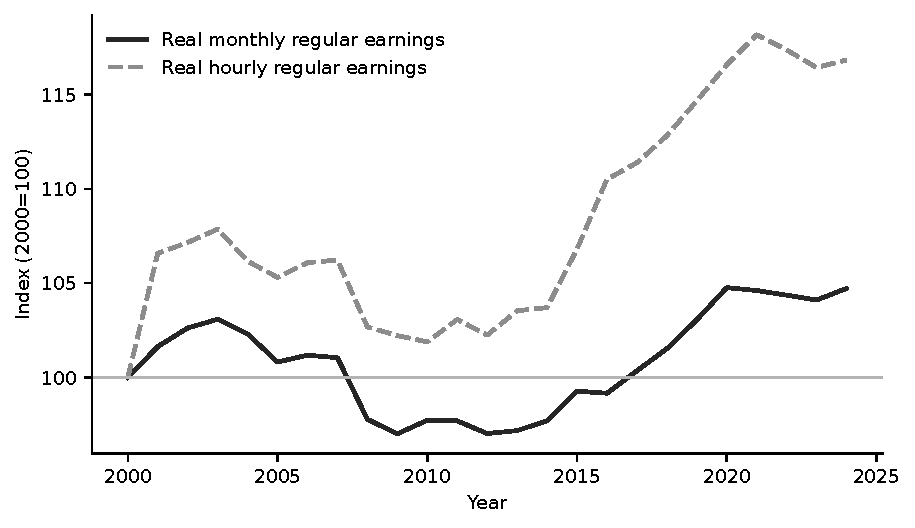
\includegraphics[width=0.92\textwidth]{figures/figure_01_real_monthly_hourly.pdf}
\caption{實質經常性月薪與時薪（共同樣本）}
\label{fig:monthly-hourly}
\begin{tabnote}[0.92\textwidth]
兩序列均以 2000 年為 100；薪資先以年度 CPI 轉為 2024 年價格。
\end{tabnote}
\end{figure}

總薪資的長期成長高於經常性薪資。實質總月薪由 55,051 元升至 61,519 元，累積對數成長 11.11\%；實質總時薪成長 21.81\%。圖~\ref{fig:regular-total} 亦顯示總薪資路徑波動較大，符合非經常性報酬受景氣與獎金影響的預期。

\begin{figure}[htbp]
\centering
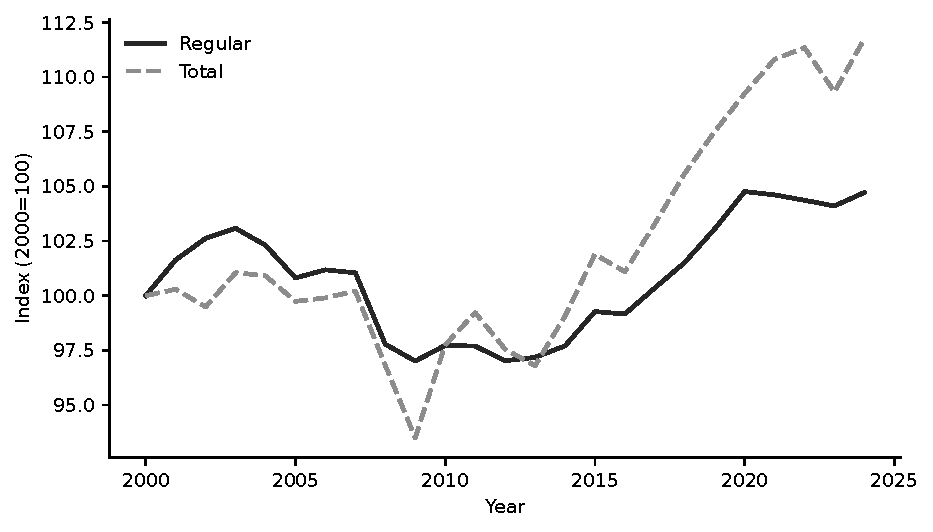
\includegraphics[width=0.92\textwidth]{figures/figure_02_regular_total.pdf}
\caption{實質經常性薪資與總薪資（共同樣本）}
\label{fig:regular-total}
\end{figure}

\subsection{主要分解}

表~\ref{tab:main} 報告實質經常性月薪的三種分解。Laspeyres 總變動 \MainTotal 元，產業內分量 \MainWithin 元，純結構分量僅 \MainShift 元，交乘為 \MainInteraction 元。Paasche 把同一交乘重新分配後，產業內為 2,118 元、結構為 $-418$ 元、交乘調整為 407 元。Törnqvist 的總對數變動為 4.611\%，其中產業內 5.094\%、結構 $-0.041$\%，殘差 $-0.441$\%。三者共同支持「產業內為主、結構較小」；但結構與交乘的個別金額依基期而變，不能把某一版本當成唯一結構效果。

\begin{table}[htbp]
\caption{2000--2024 年實質經常性月薪分解}
\label{tab:main}
\centering\small
\begin{tabular}{lrrrrr}
\toprule
方法 & 產業內 & 結構移轉 & 交乘 & 殘差 & 總變動 \\
\midrule
Laspeyres（元） & 2,525 & $-12$ & $-407$ & 0 & 2,107 \\
Paasche（元） & 2,118 & $-418$ & 407 & 0 & 2,107 \\
Törnqvist（對數百分點） & 5.094 & $-0.041$ & 0 & $-0.441$ & 4.611 \\
\bottomrule
\end{tabular}
\begin{tabnote}
共同樣本為 16 個大類。Törnqvist 為近似分解，殘差未分配至其他項。
\end{tabnote}
\end{table}

圖~\ref{fig:methods} 以各項占總變動比呈現基期敏感度。Laspeyres 與 Paasche 對結構、交乘的切分差異很大，正是完整報告交乘的理由。先分解名目薪資再以 CPI 橋接時，價格共同項吸收大部分名目成長與實質成長的差；不論順序，產業間就業占比都不是主要正向來源。

\begin{figure}[htbp]
\centering
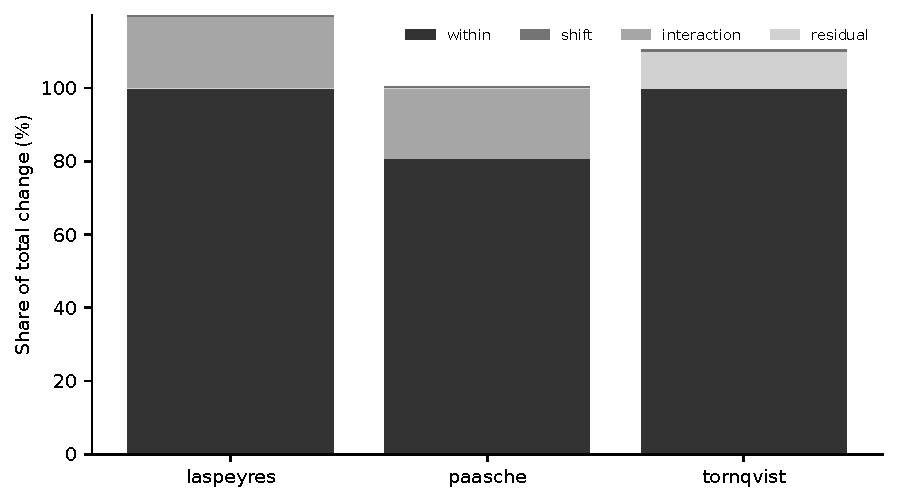
\includegraphics[width=0.88\textwidth]{figures/figure_04_decomposition_methods.pdf}
\caption{分解方法與基期敏感度}
\label{fig:methods}
\end{figure}

\subsection{分類粒度}

在第 10 次分類的 2016--2020 年共同樣本，14 個大組的 Laspeyres 產業內分量為 2,403 元，中類為 2,483 元；結構分量則由 $-62$ 元變為 $-248$ 元，交乘由 $-4$ 元變為 103 元。第 11 次分類的 2021--2024 年，粗分組產業內為 $-175$ 元，中類為 $-35$ 元；結構由 102 元變為 $-64$ 元。圖~\ref{fig:grain} 顯示，細分確實把變動重新分派，但「產業內占比隨粒度增加而下降」並未在兩段期間一致成立。因此 H2 不獲穩健支持。

\begin{figure}[htbp]
\centering
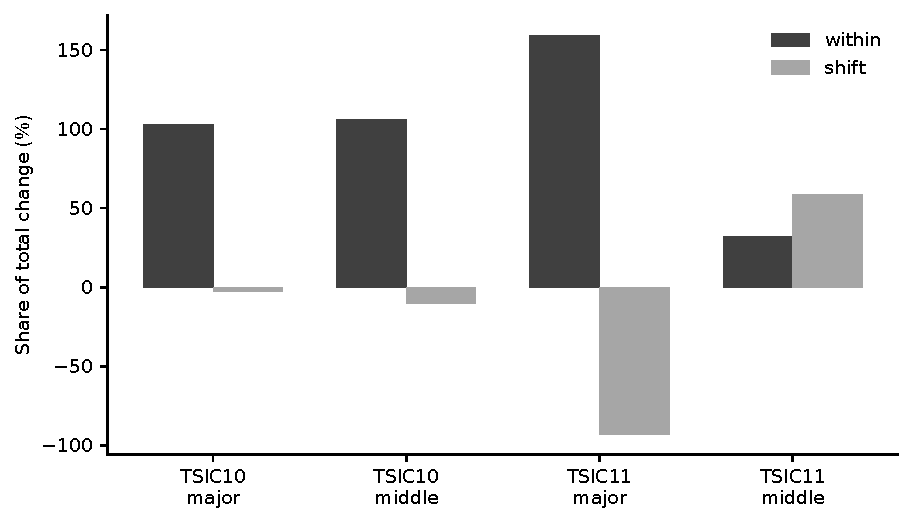
\includegraphics[width=0.9\textwidth]{figures/figure_05_granularity.pdf}
\caption{同制度共同樣本的大類與中類分解}
\label{fig:grain}
\end{figure}

\subsection{結構凍結反事實}

若固定 2000 年 16 類受僱人數占比，2024 年實質經常性月薪為 47,172 元，比實際共同樣本高 \CounterfactualGap 元（0.89\%）。固定 2008 年占比時差距只有 29 元；固定 2016 年完整 17 類占比時，反事實反而低 74 元。圖~\ref{fig:cf} 表明結構路徑不是持續同方向，且其量級小於產業內薪資變動。

\begin{figure}[htbp]
\centering
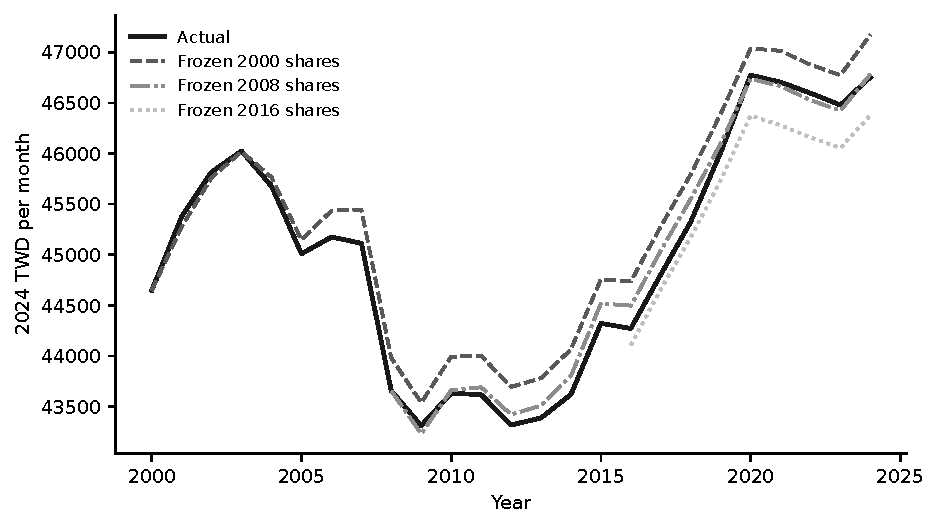
\includegraphics[width=0.9\textwidth]{figures/figure_06_counterfactual.pdf}
\caption{實際與固定受僱人數占比的反事實路徑}
\label{fig:cf}
\end{figure}

\subsection{時間路徑與不確定性}

圖~\ref{fig:shares} 顯示製造、批發零售、住宿餐飲等主要行業占比的長期移動，垂直線標示行業標準分類修訂年份。接縫與官方涵蓋變更相鄰，故本文沒有把跨制度中類跳躍直接串成經濟結構移轉。

\begin{figure}[htbp]
\centering
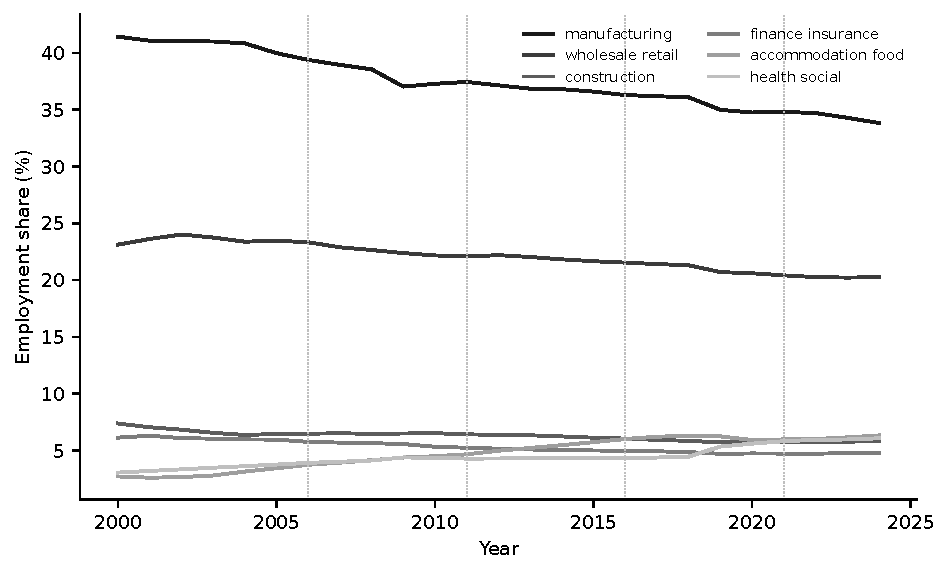
\includegraphics[width=0.92\textwidth]{figures/figure_03_employment_shares.pdf}
\caption{主要行業受僱人數占比與分類修訂}
\label{fig:shares}
\end{figure}

bootstrap 的 Laspeyres 結構分量平均為 $-22$ 元，95\% 區間為 $[-1{,}021,\,1{,}065]$ 元，雙尾 $p=\ShiftPValue$；產業內分量區間亦跨零。這些寬區間反映 25 年內景氣循環與產業共同變動的不確定性，不否定會計端點估計，而是提醒端點結果不代表一條精確、穩定的生成機制。

\subsection{年度連鎖路徑：基期敏感性大幅縮小}

結果表 10 顯示，連鎖 Laspeyres 到 2024 年的累積產業內、移轉與交乘分量分別為 \ChainWithin、\ChainShift 與 \ChainInteraction 元，合計仍精確等於 \MainTotal 元。對應的 Paasche 分量為 2,335、$-257$ 與 28 元。相較端點分解的 $\pm407$ 元交乘項，連鎖交乘絕對值縮小 \InteractionShrink\%；Laspeyres 與 Paasche 的產業內配置差也從 407 元降至 \ChainMethodGap 元。換言之，端點公式的大交乘主要是把多年同步變動一次相乘所產生的基期配置，而非一個需要獨立經濟故事的大項目。

\begin{table}[htbp]
\caption{結果表 11：連鎖分解與端點分解，2000--2024 年}
\centering\small
\begin{tabular}{llrrrr}
\toprule
方法 & 路徑 & 產業內 & 移轉 & 交乘 & 合計\\
\midrule
Laspeyres & 端點 & 2,525 & $-12$ & $-407$ & 2,107\\
Laspeyres & 年度連鎖 & 2,364 & $-229$ & $-28$ & 2,107\\
Paasche & 端點 & 2,118 & $-418$ & 407 & 2,107\\
Paasche & 年度連鎖 & 2,335 & $-257$ & 28 & 2,107\\
\bottomrule
\end{tabular}
\begin{tabnote}
單位為 2024 年新臺幣元／月。完整逐年值與未捨入恆等式見結果表 10 與 11 的 CSV。
\end{tabnote}
\end{table}

圖~\ref{fig:chained} 同時顯示觀察路徑與逐年區間。2024 年連鎖產業內分量區間為 $[-3{,}031,\,8{,}349]$ 元，移轉為 $[-1{,}565,\,659]$ 元，交乘為 $[-126,\,56]$ 元，總變動為 $[-3{,}830,\,8{,}515]$ 元。總變動區間寬度 12,345 元，大於觀察累積變動 2,107 元，故依預定規則，圖說明確標為與零不可區分。這不改寫端點會計值；它說明在只有 24 個年度差分、且景氣路徑高度相關時，重新排列區塊會產生寬廣的累積結果。

\begin{figure}[htbp]
\centering
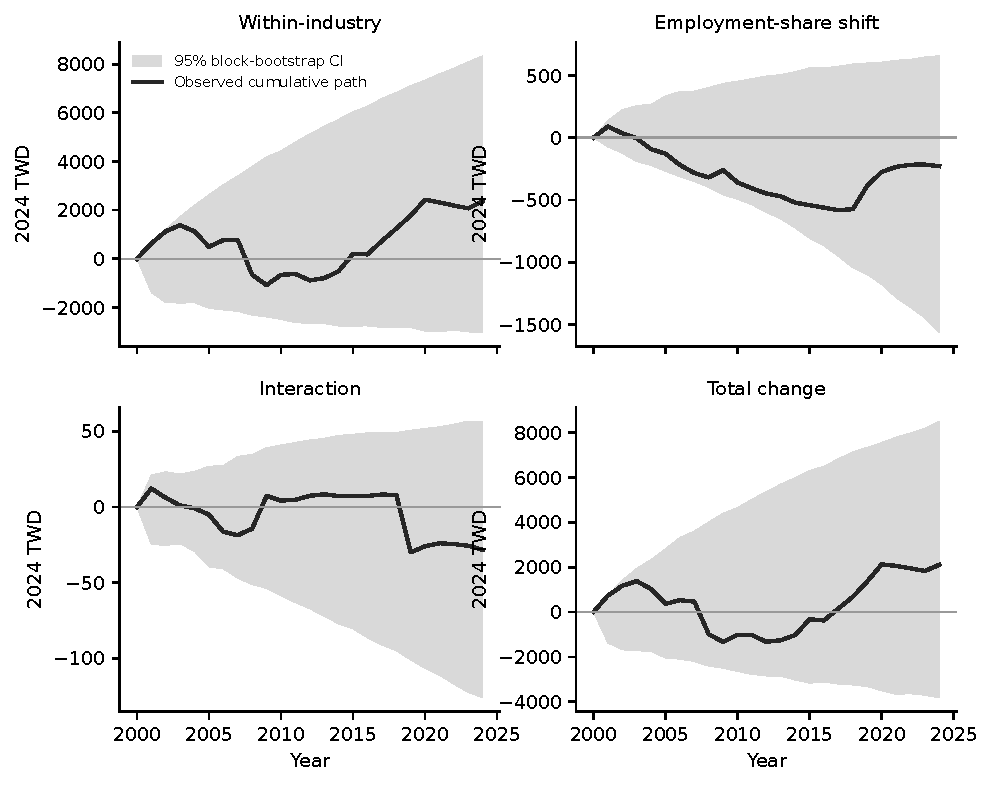
\includegraphics[width=0.96\textwidth]{figures/figure_07_chained_cumulative.pdf}
\caption{年度連鎖 Laspeyres 累積分量與三年循環區塊 bootstrap 區間}
\label{fig:chained}
\begin{tabnote}[0.96\textwidth]
陰影為 10,000 次重抽的 95\% 百分位數區間。到 2024 年，四條路徑的區間均跨零；總變動區間寬度大於累積變動絕對值，因此在此時間路徑重抽設計下與零不可區分。
\end{tabnote}
\end{figure}

\subsection{制度分段與三項條件式事前預測}

結果表 12 的六段比較顯示，2000--2002 與 2017--2020 的年平均實質經常性月薪增加最明顯，分別約 585 與 614 元；2002--2009 與 2020--2022 則為負，約 $-358$ 與 $-91$ 元。端點與連鎖的合計必然相同，但分量配置略有差異。2002--2009 的連鎖移轉為 $-295$ 元，2009--2017 為 $-282$ 元，2017--2020 轉為 138 元，2020--2022 為 48 元，2022--2024 又為 $-15$ 元。這種符號隨期間改變的模式不支持單一、恆常的結構移轉敘事。

\begin{table}[htbp]
\caption{結果表 12：制度分段的 Laspeyres 連鎖結果}
\centering\small
\begin{tabular}{lrrrr}
\toprule
期間 & 行業數 & 產業內 & 移轉 & 年平均合計\\
\midrule
2000--2002 & 16 & 1,129 & 36 & 585\\
2002--2009 & 16 & $-2,211$ & $-295$ & $-358$\\
2009--2017 & 17 & 1,803 & $-282$ & 190\\
2017--2020 & 17 & 1,715 & 138 & 614\\
2020--2022 & 17 & $-232$ & 48 & $-91$\\
2022--2024 & 17 & 169 & $-15$ & 75\\
\bottomrule
\end{tabular}
\begin{tabnote}
分量單位為 2024 年新臺幣元／月；年平均合計除以各段年數。表中省略的小交乘項仍保留在 CSV，三分量精確加總。
\end{tabnote}
\end{table}

結果表 13 對三項條件式事前預測逐項判定。第一，2019--2021 的端點 Laspeyres 移轉為 137.16 元，大於零；第二，2022--2024 為 $-14.69$ 元，方向反轉；第三，月薪與時薪累積成長差由 2019 年的 10.679 個百分點，經 2020 年 10.689，升至 2021 年 12.190，兩年皆擴大，合計增加 1.511 個百分點。三項均符合所寫方向，但它們是\textbf{條件式事前預測（研究者已觀察全期端點結果）}；本研究不以三項命中計算顯著性或聲稱真正樣本外預測成功。

\begin{table}[htbp]
\caption{結果表 13：COVID 時期條件式事前預測}
\centering\small
\begin{tabularx}{\textwidth}{p{0.9cm}p{2.4cm}Xrp{1.5cm}}
\toprule
編號 & 期間 & 可檢驗方向 & 估計 & 判定\\
\midrule
P1 & 2019--2021 & Laspeyres 移轉為正 & 137.16 元 & 支持\\
P2 & 2022--2024 & Laspeyres 移轉反轉為負 & $-14.69$ 元 & 支持\\
P3 & 2019--2021 & 月薪--時薪成長差擴大 & 1.511 點 & 支持\\
\bottomrule
\end{tabularx}
\end{table}

\subsection{產業貢獻：產業內成長並非廣泛平均}

結果表 14 把端點 Laspeyres 的產業內與移轉項拆到 16 個共同大類。製造業的產業內貢獻為 1,512 元，金融保險為 737 元，批發零售為 463 元；三者占所有產業內貢獻絕對值的 \IndustryTopThree\%，若以淨產業內總額為分母則達 107.4\%，因為營建、醫療社福、支援服務、電力燃氣等行業提供負向抵銷。製造業一項就等於淨產業內總額的 59.9\%。因此，第一階段「產業內分量占主導」不能再簡化為每個產業普遍成長；更精確的結論是，少數大型行業的正向產業內貢獻超過若干行業的負向貢獻。

\begin{figure}[htbp]
\centering
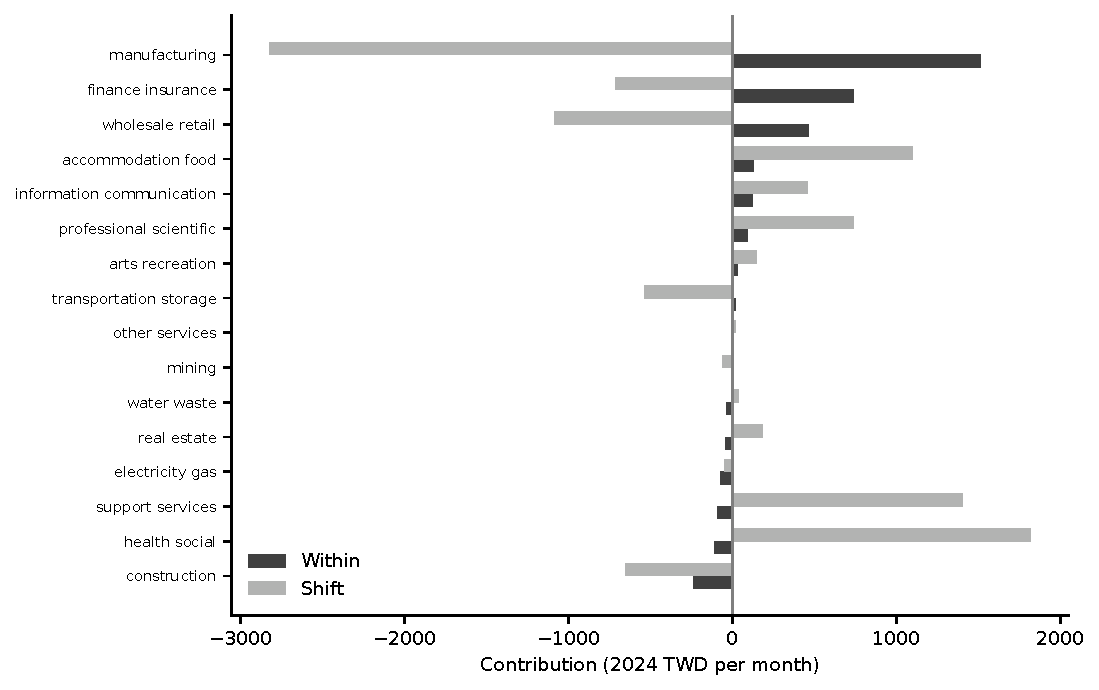
\includegraphics[width=0.94\textwidth]{figures/figure_08_industry_contributions.pdf}
\caption{16 個共同大類的產業內與就業占比移轉貢獻}
\label{fig:industry-contributions}
\begin{tabnote}[0.94\textwidth]
單位為 2024 年新臺幣元／月，依產業內貢獻排序。產業內、移轉與未畫出的交乘項各自加總後，與結果表 3 的總分量在 $10^{-10}$ 內一致。
\end{tabnote}
\end{figure}

就業占比移轉的行業分量彼此抵銷更劇烈：製造業、批發零售與金融保險的負向移轉分別約 $-2,825$、$-1,085$ 與 $-713$ 元，住宿餐飲、醫療社福、支援服務、專業科學及資訊通訊則提供正向抵銷。淨移轉僅 $-12$ 元並不表示每個行業的結構變動都小；它表示高薪與低薪行業的占比變化在這個基期權重下幾乎互相抵銷。這也解釋為何僅看總 shift 容易漏掉結構調整的方向異質性。

\subsection{總薪資：非經常性報酬改變幅度，不改主方向}

結果表 15 完整重算實質總月薪的三種分解。2000--2024 年總薪資對數成長為 \TotalGrowth\%，Laspeyres 水準增加 6,468 元，其中產業內為 8,247 元、移轉為 $-361$ 元、交乘為 $-1,419$ 元。Paasche 將同一總額配置為 6,829、$-1,779$ 與 1,419 元；Törnqvist 的對數總變動為 0.1111。總薪資仍由產業內項提供主要正向貢獻，且端點交乘依基期翻轉，與經常性薪資的質性結論一致。

總薪資相對經常性薪資多出的 4,361 元變動中，產業內差為 5,722 元、移轉差為 $-349$ 元、交乘差為 $-1,012$ 元。製造業單獨貢獻其中 2,973 元的總差，金融保險約 464 元，醫療社福約 526 元。換言之，獎金、加班費與其他非經常性給付的長期差異也高度集中，不能把總薪資成長較快解釋為所有行業一致發放更多非經常性報酬。

\begin{table}[htbp]
\caption{結果表 15：實質總月薪分解與總薪資減經常性薪資}
\centering\small
\begin{tabular}{lrrrrr}
\toprule
口徑／方法 & 產業內 & 移轉 & 交乘 & 餘差 & 合計\\
\midrule
總薪資 Laspeyres（元） & 8,247 & $-361$ & $-1,419$ & 0 & 6,468\\
總薪資 Paasche（元） & 6,829 & $-1,779$ & 1,419 & 0 & 6,468\\
總薪資 Törnqvist（對數） & 0.1289 & $-0.0150$ & 0 & $-0.0028$ & 0.1111\\
總減經常 Laspeyres（元） & 5,722 & $-349$ & $-1,012$ & 0 & 4,361\\
\bottomrule
\end{tabular}
\end{table}

結果表 16 交叉使用 2000、2001、2002 三個起點與 2022、2023、2024 三個終點。Laspeyres 總變動介於 4,970 與 6,750 元，九組產業內項全為正，九組移轉項全為負。終點 2023 因總薪資波動而給出較低總額，但沒有改變「正向產業內、負向淨移轉」的方向。這項 3 乘 3 端點檢查比只移動起點更直接呈現非經常性薪資的終點敏感性。

\subsection{工時機制與一例一休窗口}

共同樣本的加權正常工時由 2000 年每月 180.23 小時降至 2024 年 161.04 小時；加班工時由 9.85 降至 8.61 小時。圖~\ref{fig:hours} 把 16 行業路徑與加權平均並列，並以 2017、2018 兩條垂直線標出兩次制度調整。2000--2016 年正常工時平均每年下降 1.179 小時，2016--2019 年反而平均每年增加 0.024 小時；改革窗口沒有顯示正常工時下降加速。相對地，加班工時的年變化從改革前 $-0.083$ 小時變成改革窗口 $-0.251$ 小時，下降加快約 0.169 小時。行業差異很大，且窗口同時包含景氣、分類與企業調整，故不能把差值當成政策效果。

\begin{figure}[htbp]
\centering
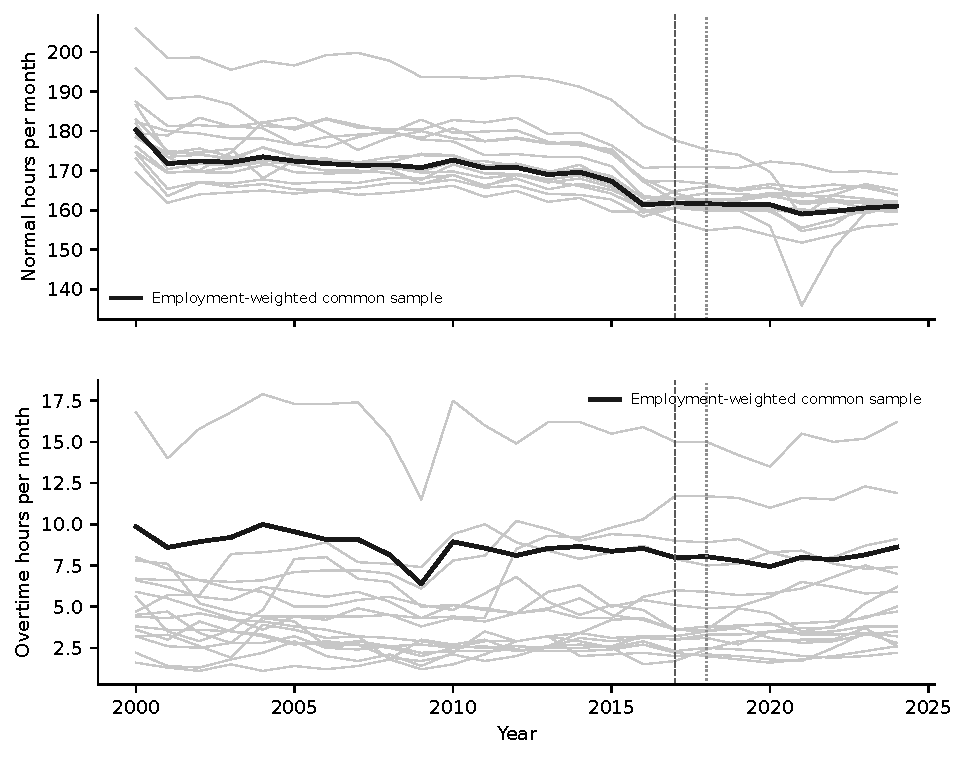
\includegraphics[width=0.96\textwidth]{figures/figure_09_hours_by_industry.pdf}
\caption{共同 16 行業的正常工時與加班工時，2000--2024 年}
\label{fig:hours}
\begin{tabnote}[0.96\textwidth]
灰線為行業，黑線為受僱人數加權平均；虛線與點線標示 2017、2018 制度年份。2016--2019 與 2000--2016 的年平均差是描述性窗口比較，不是中斷時間序列或因果估計。
\end{tabnote}
\end{figure}

兩個機制必須分開。機制 A 是分母會計：同一月薪除以較少正常工時，會得到較高經常性時薪，因此月薪與時薪成長差可由工時下降機械性擴大。機制 B 是報酬與工時組成：加班工時變動可能同時改變加班費與總薪資，但總薪資還含獎金等非工時給付，不能只用加班工時解釋。部分工時比例因無全期一致資料而未納入；本文不以任何產業占比代理。結果表 17 因此是機制相容性檢查，而非對兩個機制分別識別。

\subsection{官方發布序列與共同樣本的差距}

圖~\ref{fig:official} 比較官方發布實質序列與本文共同樣本。官方實質經常性薪資成長為 \OfficialRegularGrowth\%，共同樣本為 \MainGrowth\%，差 \RegularOfficialGap 個百分點；其中共同樣本效果為 $-0.651$ 點、官方涵蓋與大類加總效果為 $-0.003$ 點、CPI 版次效果為 $-0.001$ 點，未解釋殘差在未捨入值為零。殘差占觀察差距 0\%，未超過 30\% 警示門檻。

官方實質總薪資成長為 \OfficialTotalGrowth\%，共同樣本為 \TotalGrowth\%，差 \TotalOfficialGap 個百分點；共同樣本效果為 $-0.843$ 點、涵蓋與加總效果為 $-0.002$ 點、CPI 版次效果為 0.001 點，未解釋殘差亦為零且未觸發 30\% 警示。兩個口徑的差距幾乎全來自固定共同行業集合，而不是通膨指數選擇或程式加總誤差。這項結果同時說明共同樣本的優點與代價：它提高跨期可比性，但估計對象不再等同每年官方發布母體。

\begin{figure}[htbp]
\centering
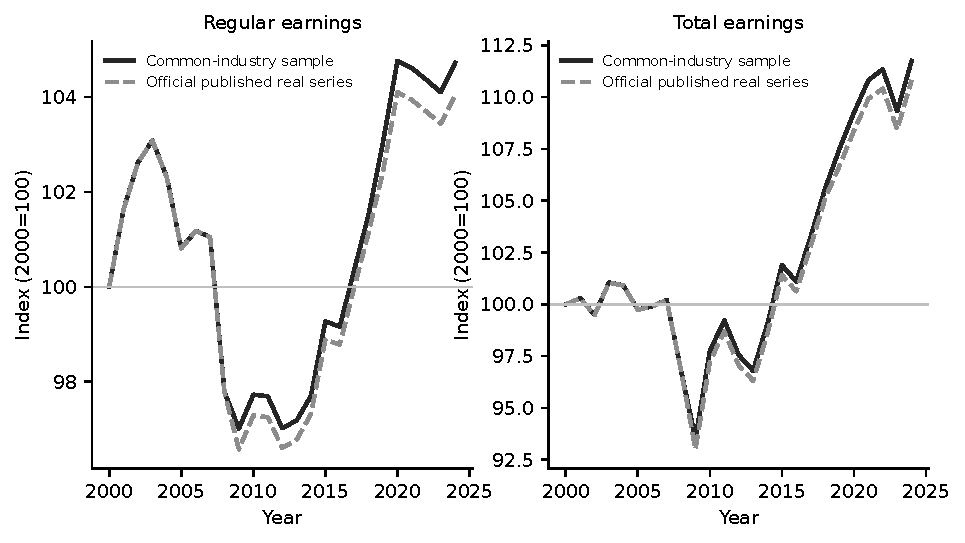
\includegraphics[width=0.95\textwidth]{figures/figure_10_official_comparison.pdf}
\caption{官方發布實質薪資與共同樣本序列}
\label{fig:official}
\begin{tabnote}[0.95\textwidth]
兩序列各自以 2000 年為 100。結果表 18 同時保留官方原基準水準、換算至 2024 年價格的水準，以及共同樣本、全行業面板與官方名目薪資按本文 CPI 平減的逐年值。
\end{tabnote}
\end{figure}

\section{限制}

第一，研究母體只涵蓋薪資及生產力統計中的工業及服務業受僱員工，不含自僱者、雇主、無酬家屬工作者、政府機關、各級一般學校與農林漁牧業。本文不能代表全體工作者的所得。

第二，官方涵蓋在 2009 與 2019 年擴增。共同樣本能避免把新增範圍當成結構移轉，但也把教育業排除在 2000 起算的主要端點分解外。2016 起算結果納入教育業，兩者母體不同，不應直接比較金額。

第三，中類年報是逐年發布版，分類內仍可能有基準修訂；本文以同年大類表驗證，並只在同一分類制度內比較。對一對多且無官方權重的跨制度對照不作主觀拆分，因此沒有單一的 2016--2024 中類長期分量。

第四，平均薪資的變化也可能來自同一產業內職業、工時型態、性別、年齡、年資與事業規模組成；大類或中類 shift-share 無法辨識這些內部組成。官方查詢介面沒有提供覆蓋 2000--2024 年的一致部分工時人數年序列，本文因此完全不使用部分工時比例，也不建立代理變數。

第五，bootstrap 使用年度時間變異，而非官方抽樣設計資訊。其區間是路徑敏感度指標，不宜解讀為母體參數的設計式信賴區間；規格不確定性則由方法、端點、粒度與涵蓋敏感度處理。最後，本文所有結果均為描述性恆等式，不支持「產業移轉導致薪資」、「一例一休造成工時變動」或「COVID 造成結構移轉」等因果語句。

\section{結論}

2000--2024 年台灣工業及服務業共同樣本的實質經常性月薪對數成長僅 4.61\%，但時薪成長 15.56\%。端點 Laspeyres 把 2,107 元變動配置為產業內 2,525 元、移轉 $-12$ 元與交乘 $-407$ 元；年度連鎖則配置為 2,364、$-229$ 與 $-28$ 元。連鎖化把基期敏感的交乘與方法差縮小 93\%，卻沒有把淨移轉改寫成主要正向來源。

第二階段修正了「產業內」的敘事邊界。前三大行業占產業內絕對貢獻 73.46\%，製造業單獨占淨產業內項 59.9\%；因此證據不是所有行業普遍溫和成長，而是少數大型行業的正貢獻抵銷多個負貢獻。總薪資雖成長較快，產業差異同樣集中。制度分段與三項條件式事前預測呈現疫情期間的正向移轉及後續反轉，但事件對齊仍不足以識別制度效果。

工時結果提供一個更直接的會計解釋：正常工時長期下降，使時薪成長機械性高於月薪；改革窗口內加班工時下降較快，但正常工時沒有比改革前趨勢下降更快。官方發布序列和共同樣本的成長差只有約 0.7 至 0.8 個百分點，且幾乎全由共同樣本界定解釋，CPI 與加總差極小。這增強了主結果的來源透明度，也提醒讀者估計對象不是每年擴張中的官方發布母體。

對政策討論而言，只用「產業升級」或「服務業化」解釋平均薪資停滯過於簡化；把端點分量當成穩定參數也同樣過度。後續研究若要回答因果問題，需要個體或事業單位縱橫資料、職業與僱用型態控制、官方抽樣共變異資訊，以及可辯護的外生變異。本文交付的是具版本、數字映射與測試的描述性基準，而不是因果終點。

\section*{資料與程式可得性}

重現入口為 \ttt{scripts/reproduce\_all.py}。來源雜湊、排除紀錄、所有論文表格 CSV、圖形、測試與 PDF 均收錄於公開 repository。官方原始資料依政府資料開放授權條款使用；程式採 MIT License。

\begin{thebibliography}{12}
\bibitem[行政院主計總處(2026a)]{dgbas-wage}
行政院主計總處（2026a），〈薪資及生產力統計〉，政府資料開放平臺，\url{https://data.gov.tw/dataset/10903}。

\bibitem[行政院主計總處(2026b)]{dgbas-class}
行政院主計總處（2026b），〈行業標準分類〉，中華民國統計資訊網，\url{https://www.stat.gov.tw/News.aspx?n=3144&sms=11195}。

\bibitem[行政院主計總處(2025)]{dgbas-yearbook}
行政院主計總處（2025），《113 年薪資與生產力統計年報》，\url{https://www.stat.gov.tw/News_Content.aspx?Create=1&n=2723&s=234856&sms=11049}。

\bibitem[行政院主計總處(2026c)]{dgbas-platform}
行政院主計總處（2026c），〈薪情平臺：薪情探索查詢系統〉，\url{https://earnings.dgbas.gov.tw/query_payroll.aspx}。

\bibitem[世界貿易組織(2026)]{wto2002}
World Trade Organization (2026), ``Separate Customs Territory of Taiwan, Penghu, Kinmen and Matsu: Member Information,'' \url{https://www.wto.org/English/thewto_e/countries_e/chinese_taipei_e.htm}.

\bibitem[International Monetary Fund(2009)]{imf2009}
International Monetary Fund (2009), \textit{World Economic Outlook: Crisis and Recovery}, \url{https://www.imf.org/en/publications/weo/issues/2016/12/31/world-economic-outlook-april-2009-crisis-and-recovery-22575}.

\bibitem[勞動部(2016)]{mol2016}
勞動部（2016），〈總統公布《勞動基準法》有關週休二日相關修正條文〉，\url{https://www.mol.gov.tw/1607/1632/1640/19791/}。

\bibitem[勞動部(2018)]{mol2018}
勞動部（2018），〈勞動基準法第 86 條：107 年修正條文自 3 月 1 日施行〉，\url{https://laws.mol.gov.tw/FLAW/FLAWDOC01.aspx?flno=86&id=FL014930}。

\bibitem[衛生福利部疾病管制署(2020)]{taiwancdc2020}
衛生福利部疾病管制署（2020），〈台灣確認首例 2019 新型冠狀病毒境外移入病例〉，\url{https://www.cdc.gov.tw/En/Category/ListContent/tov1jahKUv8RGSbvmzLwFg?uaid=pVg_jRVvtHhp94C6GShRkQ}。

\bibitem[Kitagawa(1955)]{kitagawa1955}
Kitagawa, Evelyn M. (1955), ``Components of a Difference Between Two Rates,'' \textit{Journal of the American Statistical Association}, 50(272), 1168--1194.

\bibitem[Baily et al.(1992)]{baily1992}
Baily, Martin Neil, Charles Hulten, and David Campbell (1992), ``Productivity Dynamics in Manufacturing Plants,'' \textit{Brookings Papers on Economic Activity: Microeconomics}, 187--267.
\end{thebibliography}

\appendix
\section{附錄：預先指定規格與完整輸出}

主樣本端點、敏感度期間、CPI 基期、分解公式、bootstrap 長度與亂數種子在下載資料前寫入 \ttt{PREANALYSIS.md} 並提交 Git。發現教育業在 2009 年前不可得後，只在該文件末端追加共同樣本處理，未改寫原規格。第二階段則先追加「修訂 2」並獨立提交，之後才計算連鎖、制度分段與條件式預測。下列映射是論文結果表號與 CSV 的一對一權威對照；CSV 保留未捨入數值，正文只顯示可讀位數。

\newcommand{\resultmap}[3]{#1 & \small\path{#2} & #3\\}
\begin{longtable}{p{0.8cm}p{6.3cm}p{6.2cm}}
\caption{論文結果表號與機器可讀 CSV 的一對一映射}\\
\toprule
表號 & CSV & 內容\\
\midrule
\endfirsthead
\toprule
表號 & CSV & 內容\\
\midrule
\endhead
\resultmap{01}{table_01_data_sources.csv}{資料來源、版本與涵蓋}
\resultmap{02}{table_02_external_validation.csv}{外部一致性閘門}
\resultmap{03}{table_03_main_decomposition.csv}{主端點分解}
\resultmap{04}{table_04_granularity_comparison.csv}{大類與中類粒度}
\resultmap{05}{table_05_monthly_hourly.csv}{月薪與時薪}
\resultmap{06}{table_06_regular_total.csv}{經常性與總薪資}
\resultmap{07}{table_07_period_sensitivity.csv}{起點敏感度}
\resultmap{08}{table_08_counterfactual.csv}{固定占比反事實}
\resultmap{09}{table_09_inference.csv}{端點區塊 bootstrap}
\resultmap{10}{table_10_chained_decomposition.csv}{年度連鎖路徑與區間}
\resultmap{11}{table_11_chained_vs_endpoint.csv}{連鎖與端點比較}
\resultmap{12}{table_12_institutional_periods.csv}{制度分段}
\resultmap{13}{table_13_covid_predictions.csv}{條件式事前預測}
\resultmap{14}{table_14_industry_contributions.csv}{16 行業貢獻}
\resultmap{15}{table_15_total_wage_decomposition.csv}{總薪資與口徑差}
\resultmap{16}{table_16_total_wage_endpoint_sensitivity.csv}{總薪資九組端點}
\resultmap{17}{table_17_hours_mechanism.csv}{工時路徑與資料可用性}
\resultmap{18}{table_18_official_comparison.csv}{官方發布序列比較}
\bottomrule
\end{longtable}

\end{document}

